\documentclass[11pt]{article}
\usepackage[utf8]{inputenc}
\usepackage[francais]{babel}
\usepackage{graphicx} 
\usepackage{geometry}
\usepackage{fancyhdr}
\usepackage{amssymb}

\geometry{hmargin=2.5cm, vmargin=2.5cm}

\def\blurb{TDDC17 - Lab 2 : Search (Java version)}

\def\ligne#1{%
  \hbox to \hsize{%
    \vbox{\centering #1}}}%

\makeatletter
\def\maketitle{%
	\pagestyle{empty}
	\vbox{\centering Linköping University\\
	IDA - The Department of Computer and Information Science}
	\vfill
	\vbox{\centering \Large \@title}
	\vspace{5mm}
	\vbox{\centering \Large \@author}
	\vfill
	\vbox{\centering \@date}
	\clearpage
}

\title{Lab 2 : Search (Java version)}
\author{Simon Vernhes}
\date{\today}

\begin{document}
  \pagestyle{fancyplain}
  \setlength{\parskip}{.6ex plus .4ex minus .4ex}
  \renewcommand{\headrulewidth}{0pt}
  \renewcommand{\footrulewidth}{0.6pt}
  \fancyhf{}
  \fancyhead{}
  \lfoot{\blurb}
  \rfoot{Page \thepage}


  \maketitle \clearpage
  \setlength{\parskip}{2ex plus .4ex minus .4ex}

  \pagestyle{plain}
  \setcounter{page}{1}

  \section{States and Actions}
In the vacuum cleaner domain, the states are all moving element in the world, so a state can be describe by :
\begin{itemize}
  \item the vaccum cleaner position (x, y)
  \item his direction
  \item the cell is withy or not
\end{itemize}

All other things in this world like walls, home position are static and so are the same for all states.

The actions in this world is simple all the action that the vacuum cleaner can do : 
\begin{itemize}
  \item turn right
  \item turn left
  \item move forward
  \item suck dirt
  \item stop
\end{itemize}

The sensors of the vacuum cleaner are not actions.


  \section{Breadth First Search and Uniform Cost Search}
There's no difference between BFS and UCS when the cost of each action is 1 because UCS explore the (unexplored) node which is the nearest from the start node. It will result that the UCS will explore the tree level by level starting by the top node. So it's exactly the same exploration as BFS.

If, at first goal depth, there is more than 1 goal, then the algorithm may return different path but will get the same score (depending on the way the two algorithm select actions which will lead to the same cost).

  \subsection{Results}
So, in this world, we can observe that BFS and UCS always get the same score.

They don't choose exactly the same path because we can see that BFS suck dirt first and that UCS suck dirt just before leaving a cell.
So, in that case UCS seams to explore more nodes than BFS but they obviously stop exploration at the same depth of the tree.


  \section{A* heuristic}
In the vacuum domain, the heuristic fonction for A* to go the a cell(x1, y2) to a goal(x2, y2 could be the manhanttan distance :
                                                                                
$h(currentCell) = \|goal - currentCell\| =  |x2 - x| + |y2 - y|$

The cost function g is simply the number of action done to go the current cell.

This heuristic is an admissble heuristic because it will always be the no-more than the lowest-cost path to the goal. The vaccum agent can just go to a cell which is on the top or right or bottom or left of his current position, that made that the manhattan distance give the lowest-cost path to the goal.

However, this heuristic don't consider that the agent have to turn before go forward to another cell. Anyway, the lowest-cost path became the h(x) + 1 (the cost of 1 turn).


  \section{Duplicate-checking}
  \subsection{Breadth First Search}
Using duplicate-checking in Breadth First Search will cut off some branches in the exploration tree. So the exploration will become faster. Anyway, BFS explore the tree level by level, so in that case the algorithm will find a solution with or without these cuts, because of the completeness of this algorithm. Moreover, using duplicate-checking will not change the complexity of the algorithm.

After a test on a 1x2 environment with a dirt cell (the cell where the agent is not initially), we can see that the algorihm expanded 170 nodes with a path cost of 7. If this algorithm expended all node without duplicate-checking, it should have expended at least $(\sum_{n=0}^{6} 4^n) + 1 = 5462$ nodes. So the provided algorithm implement duplicate-checking.

  \subsection{Depth First Search}
Using duplicate-checking in Depth First Search will really improve this algorithm. By exemple, in the vacuum domain, if the actions are always choosen in the same order (starting by turn left), then the algorithm will just going deep (always choosing to turn left) in the tree exploring only tiny posibilities and never try to suck something so it will never go to a goal (except if initialy there's no dirt). With duplicate checking, the algorithm will stop after 4 turn left and then explore another part of the tree and finally found a solution.

If the actions are not always choosen in the same order, then the algorithm might found a goal, but it the algorithm will still explore a enormous tree.

After some test, we can see that the provided DFS algorithms always go in infinite computation, so it does not implement duplicate-checking.


  \section{Choosing actions}
As we've seen before, Depth First search is affected by the way we choose the action to perform.

Breadth First Search and Uniform Cost Search will not be really affected because they will return a path with the same cost.


  \section{A* and Greedy Search}
These two heuristic are not admissible.

For H1, by example if there's two dirt square in a $1x2$ world, and if you are on cell which is not the home cell and in the direction to the home cell, you need 3 moves to go to the goal (suck, go forward, suck). But H1 will return $2^2 = 4$. That means that H1 is not an admissible heuristic.

For H2, by example, in a $1x2$ world, if the not-home cell is dirty and you're on it (and in direction to the home cell), you need $2$ moves to go to the goal (suck, go forward). But H2 will return $1^2 + (1+1)*1 = 3$. That means that H2 is not an admissible heuristic.

Anyway, using the Greedy algorithm with heuristic H1 seems to never lead to a goal node. That's seems understandable because this heuristic give really often the same result. So the don't help greedy algorithm to choose the good action. Sometimes this algorithm with H1 found a path to goal node, so maybe there's a random selection between action which have the same value for heuristic H1.

A* seems to be better than Greedy with heuristic H1. It's obviously because A* don't forget the past, and know the cost of the current past. So with a bad heuristic like H1, A* could seems a bit like a Breadth First Search.

Greedy algorithm with heuristic H2 give better result than with H1. It's because this heuristic H2 suits better to this world and so greedy algorithm go faster to the goal node. 

Sometimes, using the heuristic H2, Greedy will take too much time (and too much memory) (usually in big worlds). In that case, A* will most of the time found a path in acceptable time.

Anyway, in small world, Greedy will be faster (because he only care of being the nearest possible of the goal node, not taking care of the past).


  \section{Algorithms}
  \subsection{A*}
A* use a function to determine the order in which the search visits nodes in the tree. This function is $f(x) = g(x) + h(x)$ where $g(x)$ is the path cost from the starting node to the current node and $h(x)$ is an admissible heuristic function. A* choose the next unvisited node where the function $f(x)$ is the minimum.
  
An admissible heuristic function means if $h(x) \leq r(x)$ where $r(x)$ is the cost of the path between the node $x$ and the goal node. In the vacuum world, to search a path between a cell to another, an admissible heuristic could be the Manhattan distance.

Let's take the graph below. We want to go from node A to node D. An admissible function h could be :
$h(B) = 12$,
$h(C) = 7$,
$h(D) = 0$,
$h(E) = 10$,
$h(F) = 2$,
$h(G) = 5$

\begin{figure}[!h]
  \centering
  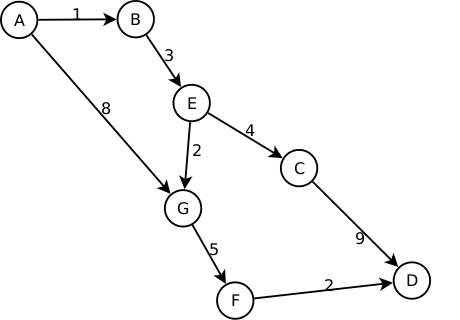
\includegraphics[height=6cm]{img/AStar_exemple.png}
  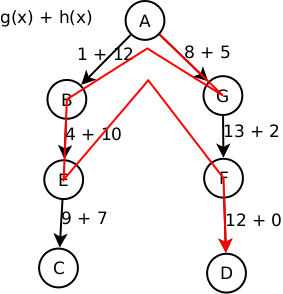
\includegraphics[height=6cm]{img/AStar_tree.png}
  \caption{Graph and it's A* exploration tree}
  \label{BFS_Levels}
\end{figure} 

Here we can see that the solution is not optimal. It's because the heuristic is not consistent ( $h(B) > cost(B,E) + h(C)$).

Using a consistent heuristic with A* assure to find the optimal path.

  \subsection{Breadth First Search}
BFS will explore the graph using a queue (FIFO), that imply that node who are the nearest (not in real cost, but in number of nodes to go across) will be explore first. The graph will be explored level by level.
We can see this exploration on the image below :

\begin{figure}[!h]
  \centering
  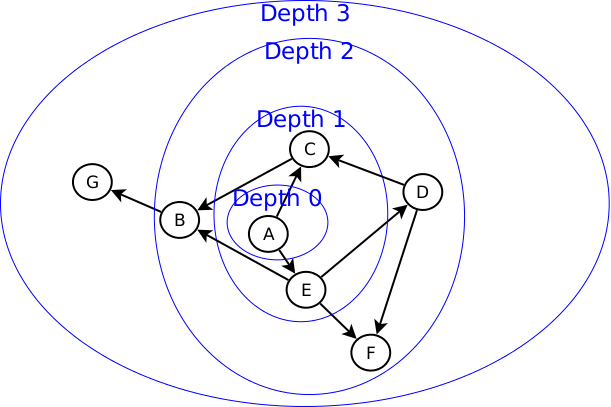
\includegraphics[height=8cm]{img/BFS_Levels.png}
  \caption{BFS exploration levels}
  \label{BFS_Levels}
\end{figure} 

Here are the way how BFS explore the tree.

\begin{figure}[h!]
  \centering
  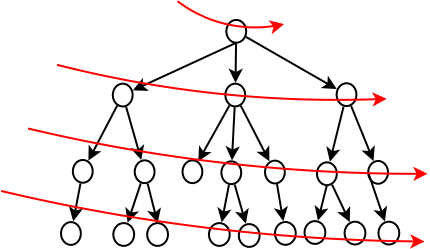
\includegraphics[height=6cm]{img/BFS_explo.png}
  \caption{BFS exploration}
\end{figure} 

BFS is a blind-search algorithm, so he don't take of the path cost during his exploration.

  \subsection{Iterative Depth First Search}

The Iterative deepening search algorithm is an extension to the Depth Limited Search algorithm.

This algorithm start with a depth threshold of 1 and execute a Depth Limited Search algorithm. If no goal node has been found, then the algorithm increase the depth threshold and re-execute a Depth Limited Search with this new threshold. The algorithm iterate until he found a goal node. Here are the way how Iterative Deepening explore the tree.

\begin{figure}[h!]
  \centering
  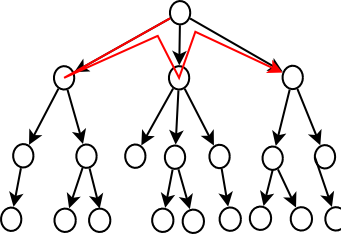
\includegraphics[height=4cm]{img/Ite_explo1.png}
  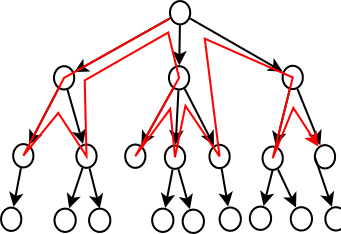
\includegraphics[height=4cm]{img/Ite_explo2.png}
  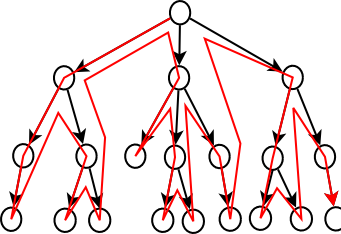
\includegraphics[height=4cm]{img/Ite_explo3.png}
  \caption{Iterative deepening (Depth threshold respectively 1, 2 and 3)}
\end{figure} 

Iterative Deepening Search is also a blind-search algorithm, so he don't take of the path cost during his exploration.

\clearpage

  \section{Completeness and Optimality}
  \subsection{Breadth First Search}
\begin{itemize}
  \item \textbf{Complete} because BFS expand node level-by-level in the tree, so the shallowest goal is at depth d, BFS will expand it when expending node of depth d.
  \item \textbf{Optimal} if all the steps cost are equals.
\end{itemize}

  \subsection{Uniform-cost search}
\begin{itemize}
  \item \textbf{Complete} 
  \item \textbf{Optimal}
\end{itemize}

If all the cost are positive, then the cost of the path can only grows, this ensure completeness and also optimality.

  \subsection{Depth-first search}
\begin{itemize}
  \item \textbf{Non complete} (can be complete if duplicate-checking is implemented in a finite graph) 
  \item \textbf{Non optimal} because these algorithm explore some deep nodes before shallow ones so it can found a deeper goal node than the shallowest goal node.
\end{itemize}

  \subsection{Depth-limited search}
\begin{itemize}
  \item \textbf{Non Complete} (can be complete if the limited depth is lesser than the depth of the shallowest goal node)
  \item \textbf{Non Optimal} see DFS
\end{itemize}

  \subsection{Iterative deepening DFS}
\begin{itemize}
  \item \textbf{Complete} Because there will be an iteration where the depth limit will become greater than the depth of the shallowest goal node.
  \item \textbf{Optimal} if all the steps cost are equals.
\end{itemize}

  \subsection{A*}
\begin{itemize}
  \item \textbf{Complete} if the heuristic is admissible 
  \item \textbf{Optimal} if the heuristic is consistent
\end{itemize}


  \section{Back to lab 1}

We can't really use an offline search during lab1 because we doesn't know anything about the world. We just know what sensor tell us, and what we learn about the world before. So we can't generate a path to achieve the goal at the beginning.

Anyway, after exploring a bit the world, we can use a search algorithm to lead the vacuum agent from a cell to another. During the lab1, I used a Dijkstra algorithm to do that. It would be easy to change this Dijkstra to an A* because we just have to add the heuristic, which will be the manhanttan distance.


\end{document} 

